\documentclass[
    11pt, % The default document font size, options: 10pt, 11pt, 12pt
%codirector, % Uncomment to add a codirector to the title page
]{charter}


% El títulos de la memoria, se usa en la carátula y se puede usar el cualquier lugar del documento con el comando \ttitle
\titulo{Predicción de series de tiempos aplicado al trading de criptomonedas usando la arquitectura de Transformers}

% Nombre del posgrado, se usa en la carátula y se puede usar el cualquier lugar del documento con el comando \degreename
%\posgrado{Carrera de Especialización en Sistemas Embebidos}
%\posgrado{Carrera de Especialización en Internet de las Cosas} 
\posgrado{Carrera de Especialización en Inteligencia Artificial}
%\posgrado{Maestría en Sistemas Embebidos} 
%\posgrado{Maestría en Internet de las cosas}

% Tu nombre, se puede usar el cualquier lugar del documento con el comando \authorname
% IMPORTANTE: no omitir titulaciones ni tildación en los nombres, también se recomienda escribir los nombres completos (tal cual los tienen en su documento)
\autor{Martín Leonardo Centurión}

% El nombre del director y co-director, se puede usar el cualquier lugar del documento con el comando \supname y \cosupname y \pertesupname y \pertecosupname
\director{Director a definir}
\pertenenciaDirector{pertenencia}
\codirector{} % para que aparezca en la portada se debe descomentar la opción codirector en los parámetros de documentclass
\pertenenciaCoDirector{FIUBA}

% Nombre del cliente, quien va a aprobar los resultados del proyecto, se puede usar con el comando \clientename y \empclientename
\cliente{Nombre del cliente}
\empresaCliente{Empresa del cliente}

\fechaINICIO{15 de octubre de 2024}        %Fecha de inicio de la cursada de GdP \fechaInicioName
\fechaFINALPlan{03 de diciembre de 2024}    %Fecha de final de cursada de GdP
\fechaFINALTrabajo{diciembre de 2025}    %Fecha de defensa pública del trabajo final


\begin{document}

    \maketitle
    \thispagestyle{empty}
    \pagebreak


    \thispagestyle{empty}
    {\setlength{\parskip}{0pt}
    \tableofcontents{}
    }
    \pagebreak


    \section*{Registros de cambios}
    \label{sec:registro}


    \begin{table}[ht]
        \label{tab:registro}
        \centering
        \begin{tabularx}{\linewidth}{@{}|c|X|c|@{}}
            \hline
            \rowcolor[HTML]{C0C0C0}
            Revisión & \multicolumn{1}{c|}{\cellcolor[HTML]{C0C0C0}Detalles de los cambios realizados} & Fecha      \\ \hline
            0        & Creación del documento                                                          & \fechaInicioName \\ \hline
            1        & Primera entrega                                                          & 30 de octubre de 2024 \\ \hline
%1      & Se completa hasta el punto 5 inclusive                & {día} de {mes} de 202X \\ \hline
%2      & Se completa hasta el punto 9 inclusive
%		  Se puede agregar algo más \newline
%		  En distintas líneas \newline
%		  Así                                                    & {día} de {mes} de 202X \\ \hline
%3      & Se completa hasta el punto 12 inclusive                & {día} de {mes} de 202X \\ \hline
%4      & Se completa el plan	                                 & {día} de {mes} de 202X \\ \hline

% Si hay más correcciones pasada la versión 4 también se deben especificar acá

        \end{tabularx}
    \end{table}

    \pagebreak



    \section*{Acta de constitución del proyecto}
    \label{sec:acta}

    \begin{flushright}
        Buenos Aires, \fechaInicioName
    \end{flushright}

    \vspace{2cm}

    Por medio de la presente se acuerda con \authorname\hspace{1px}que su Trabajo Final de la \degreename\hspace{1px}
    se titulará ``\ttitle'' y consistirá en la implementación de un sistema de predicción de series de tiempos
    aplicado al trading de criptomonedas usando la arquitectura de Transformers.
    El trabajo tendrá un presupuesto preliminar estimado de 600
    horas y un costo estimado de \$37.500.000, con fecha de inicio el \fechaInicioName\hspace{1px}
    y fecha de presentación pública en \fechaFinalName.

    Se adjunta a esta acta la planificación inicial.

    \vfill

% Esta parte se construye sola con la información que hayan cargado en el preámbulo del documento y no debe modificarla
    \begin{table}[ht]
        \centering
        \begin{tabular}{ccc}
            \begin{tabular}[c]{@{}c@{}}
                Dr. Ing. Ariel Lutenberg \\ Director posgrado FIUBA
            \end{tabular} & \hspace{2cm} &
            \begin{tabular}[c]{@{}c@{}}
                \clientename \\ \empclientename
            \end{tabular} \vspace{2.5cm} \\
            \multicolumn{3}{c}{\begin{tabular}[c]{@{}c@{}}
                                   \supname \\ Director del Trabajo Final
            \end{tabular}} \vspace{2.5cm} \\
        \end{tabular}
    \end{table}


    \section{1. Descripción técnica-conceptual del proyecto a realizar}
    \label{sec:descripcion}
    Este es un proyecto personal con el objetivo de estudiar, en el contexto de análisis y predicción de series de tiempo,
    el desempeño de la arquitectura de Transformers. Esta tecnología es una pieza fundacional del estado del arte actual
    en deep learning en general y en predicción de series de tiempos en particular.

    Para dicho estudio se propone la aplicación a un sistema de trading de criptomonedas con el cual se espera obtener
    rendimiento y, al mismo tiempo, regular el nivel de riesgo incurrido.

    Es valioso explorar el uso de Transformers y sus variantes, ya que permitiría obtener una ventaja comparativa con
    respecto a otras soluciones mediante la utilización de nuevos modelos basados que presenten mejor poder de predicción.

    El objetivo del trading consiste en obtener una ganancia comprando instrumentos, en este caso criptomonedas, a un precio menor al que se los vende.
    Se caracteriza por tener un plazo de tiempo acotado, ya que, en el largo plazo las fluctuaciones del mercado pierden relevancia
    frente a las condiciones fundamentales del instrumento en cuestion.
    Esto es: el precio del bitcoin (BTC) de hoy a diez años depende más de tendencias macroeconómicas que de otras fluctuaciones.
    Al otro extremo está el trading de alta frecuencia donde se realizan varias operaciones por segundo y requiere del uso de hardware y redes especializadas.
    Por lo dicho anteriormente se decide acotar el plazo de predicción entre un minuto y una semana.

    El resultado final, como ilustra la figura \ref{fig:diagBloques}, constara de un sistema capaz de comprar y vender criptomonedas de forma autónoma consultando
    un modelo preentrenado con datos históricos cotizaciones pertinentes.

    \begin{figure}[htpb]
            \centering
            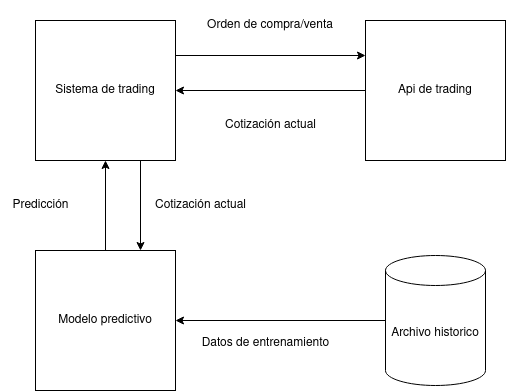
\includegraphics[width=.65\textwidth]{./Figuras/bloques-tp-final.drawio.png}
            \caption{Diagrama en bloques del sistema.}
            \label{fig:diagBloques}
        \end{figure}

    \newpage
    \section{2. Identificación y análisis de los interesados}
    \label{sec:interesados}

    \begin{table}[ht]
        \begin{tabularx}{\linewidth}{@{}|l|X|X|l|@{}}
            \hline
            \rowcolor[HTML]{C0C0C0}
            Rol         & Nombre y Apellido & Organización  & Puesto                     \\ \hline
            Responsable & \authorname       & FIUBA         & Alumno                     \\ \hline
            Orientador  & \supname          & \pertesupname & Director del Trabajo Final \\ \hline
        \end{tabularx}
        \label{tab:interesados}
    \end{table}
    \begin{itemize}
        \item Orientador: \supname  a definir.
        \item Responsable: El alumno encargado de llevar a cabo la planificación e implementación.
    \end{itemize}


    \section{3. Propósito del proyecto}
    \label{sec:proposito}
    El propósito de este proyecto es la investigación y aplicación de arquitecturas de Transformers para el trading de criptomonedas.
    Se buscará explorar esta nueva tecnología y comparar su desempeño con otros modelos previamente utilizados en la industria.


    \section{4. Alcance del proyecto}
    \label{sec:alcance}
    El proyecto incluye:
    \begin{itemize}
        \item El desarrollo de un sistema que realice trading de criptomonedas de forma no supervisada.
        \item Análisis y visualización de los datos históricos correspondientes a las cotizaciones de las criptomonedas seleccionadas.
        \item La exploración de modelos del estado del arte para el análisis y predicción de series de tiempo.
        \item El rango temporal máximo a predecir es de una semana.
        \item El rango temporal mínimo a predecir no implica el uso de hardware especializado ni la conexión a redes especiales.
    \end{itemize}
    El proyecto no incluye:
    \begin{itemize}
        \item Un servicio ni una API para exponer el modelo.
        \item Aprovisionamiento infraestructura para correr el modelo.
        \item Implementación de un modelo.
    \end{itemize}


    \section{5. Supuestos del proyecto}
    \label{sec:supuestos}
    Para el desarrollo del presente proyecto se supone que:

    \begin{itemize}
        \item Existen API's con las cuales integrarse para realizar el trading.
        \item Existen datasets históricos para entrenar los modelos.
        \item La arquitectura de transformers es efectiva para la predicción de series de tiempo.
        \item Existen modelos adecuados para entrenarlos.
    \end{itemize}

    \section{6. Requerimientos}
    \label{sec:requerimientos}

    \begin{enumerate}
    \item Requerimientos funcionales:
      \begin{enumerate}
      \item El sistema debe poder operar de de forma autónoma.
      \item El usuario debe poder ingresar credenciales de una cuenta en un exchange de criptomonedas con la cual operar.
      \item El sistema debe poder detenerse de forma segura.
      \item El sistema debe tener criterios configurables que determinen el nivel tolerable de riesgo, para un criterio de riesgo a definir.
      \item Al sistema se le puede definir un monto máximo con el cual operar.
      \end{enumerate}
    \item Requerimientos de documentación:
      \begin{enumerate}
      \item Debe estar documentado como iniciar y detener el sistema de forma segura.
      \item Debe estar documentado los parámetros de configuración y como afectan al comportamiento del sistema.

      \end{enumerate}
    \item Requerimiento de testing:
      \begin{enumerate}
      \item El sistema contara con tests de integración contra la API del exchange elegido.
      \item El sistema contara con tests de componente validando las reglas de negocio del servicio. Por ejemplo: respetar el monto máximo o el limite de riesgo.
      \item El modelo sera evaluado según su capacidad predicativa teniendo en cuenta los datos históricos disponibles.
      \item Se diseñara una forma de monitorizar el rendimiento del sistema.
      \end{enumerate}

    \item Requerimientos de la interfaz:
      \begin{enumerate}
      \item El sistema proveerá una interfaz de linea de comandos(CLI) para iniciar y detener el sistema.
      \item La CLI sera clara en sus errores cuando faltase información necesaria para iniciar el sistema.
      \end{enumerate}

    \end{enumerate}

    \section{7. Historias de usuarios (\textit{Product backlog})}
    \subsection{Roles}
    Se identifican los siguientes roles:
    \begin{itemize}
    \item Inversor: individuo registrado en el exchange que aporta la cuenta con capital disponible para operar.
    \item Ingeniero de Operaciones: individuo con conocimientos técnicos responsable de poner el sistema en marcha y velar por su correcto funcionamiento.
    \item Gerente de inversiones: individuo encargado de decidir los parámetros con los cuales se configurara el sistema en base a los objetivos de negocio.
    \end{itemize}

    \label{sec:backlog}
    \subsection{Product backlog}
    \subsubsection{Inversor}
    \begin{enumerate}
    \item \textbf{Como} inversor \textbf{quiero} proveer de forma secura las credenciales de mi cuenta \textbf{para} que se pueda operar con el capital disponible.
      \textit{Story points}: 3  (complejidad: 1, dificultad: 1, incertidumbre: 1)
    \end{enumerate}

    \subsubsection{Ingeniero de Operaciones}
    \begin{enumerate}
    \item \textbf{Como} ingeniero de operaciones \textbf{quiero} poder levantar el sistema \textbf{para} corroborar que no haya errores de configuración.
      \textit{Story points}: 3  (complejidad: 1, dificultad: 1, incertidumbre: 1)
    \item \textbf{Como} ingeniero de operaciones \textbf{quiero} poder iniciar el sistema \textbf{para} que empiece a operar.
      \textit{Story points}: 7  (complejidad: 2, dificultad: 2, incertidumbre: 3)
    \item \textbf{Como} ingeniero de operaciones \textbf{quiero} poder detener el sistema \textbf{para} que deje de operar.
      \textit{Story points}: 3  (complejidad: 1, dificultad: 1, incertidumbre: 1)
    \item \textbf{Como} ingeniero de operaciones \textbf{quiero} poder detener el sistema de forma segura \textbf{para} que no queden transacciones sin finalizar.
      \textit{Story points}: 5  (complejidad: 3, dificultad: 1, incertidumbre: 1)
    \item \textbf{Como} ingeniero de operaciones \textbf{quiero} poder matar el sistema \textbf{para} que deje consumir recursos.
      \textit{Story points}: 1  (complejidad: 1, dificultad: 1, incertidumbre: 1)
    \item \textbf{Como} ingeniero de operaciones \textbf{quiero} ver logs del sistema  \textbf{para} monitorizar errores.
      \textit{Story points}: 1  (complejidad: 1, dificultad: 1, incertidumbre: 1)
    \end{enumerate}

    \subsubsection{Gerente de inversiones}
    \begin{enumerate}
    \item \textbf{Como} gerente de inversiones  \textbf{quiero} configurar el nivel de riesgo \textbf{para} evitar la perdida de capital.
      \textit{Story points}: 6  (complejidad: 1, dificultad: 2, incertidumbre: 3)
    \item \textbf{Como} gerente de inversiones \textbf{quiero} configurar un limite de dinero a invertir \textbf{para} evitar la perdida de capital.
      \textit{Story points}: 5  (complejidad: 1, dificultad: 2, incertidumbre: 2)
    \end{enumerate}

    \section{8. Entregables principales del proyecto}
    \label{sec:entregables}

    Los entregables del proyecto son:

    \begin{itemize}
    \item Documentación.
    \item Código fuente.
    \item Memoria del trabajo final.
    \end{itemize}

    \section{9. Desglose del trabajo en tareas}
    \label{sec:wbs}


    \begin{enumerate}
    \item Estudio del dominio del problema (176 h):
      \begin{enumerate}
      \item Búsqueda de bibliografía (8 h).
      \item Estudio sobre trading (40 h).
      \item Estudio sobre indicadores y análisis técnico (40 h).
      \item Estudio sobre trading algorítmico (30 h).
      \item Estudio sobre análisis de series de tiempo (48 h).
      \item Estudio sobre compra/venta de criptomonedas (10 h).
      \end{enumerate}

    \item Procuración y análisis de datos (38 h):
      \begin{itemize}
      \item Obtención de datos (3 h).
      \item Análisis y tratamiento (10 h).
      \item Exploración y visualización inicial (15 h).
      \item Entrenamiento y selección de un modelo simple para hacer de base (10 h).
      \end{itemize}

    \item Exploración de métodos tradicionales y estado del arte (150 h):
      \begin{enumerate}
      \item Métodos tradicionales: Moving averages, autoregresión, ARIMA, State Space Models, etc. (50 h).
      \item Estado del arte: RNN, CNN, Hybrids, Prophet, DeepAR, etc. (50 h).
      \item Entrenamiento y selección de modelos (30 h).
      \item Visualización y exploración (20 h).
      \end{enumerate}

    \item Exploración del uso de transformers en series de tiempo (100 h):
      \begin{enumerate}
      \item Investigación redes neuronales, transformers, estado del arte, etc. (20 h).
      \item Entrenamiento y selección de modelos (50 h).
      \item Visualización y exploración (20 h).
      \item Comparativa con estado del arte (10 h).
      \end{enumerate}

    \item Implementación del sistema de trading (100 h):
      \begin{enumerate}
      \item Integración con la API del exchange para compra/venta (20 h).
      \item Parametrización de las variables riesgo, monto a operar, etc. (15 h).
      \item Integración con la API del exchange para cotizaciones (15 h).
      \item Implementación de la lógica de decisión de compra/venta (15 h).
      \item Integración con el modelo (10 h).
      \item Productización de la CLI (15 h).
      \item Desarrollo de la lógica de monitorización del rendimiento (20 h).
      \item Documentación (5 h).
      \end{enumerate}

    \item Escritura de las memorias (50 h).
    \end{enumerate}

    Cantidad total de horas: 614.
    \section{10. Diagrama de Activity On Node}
    \label{sec:AoN}

    \begin{consigna}{red}
        Armar el AoN a partir del WBS definido en la etapa anterior.

        Una herramienta simple para desarrollar los diagramas es el Draw.io (\url{https://app.diagrams.net/}).
        \href{https://app.diagrams.net}{Draw.io}


        \begin{figure}[htpb]
            \centering
            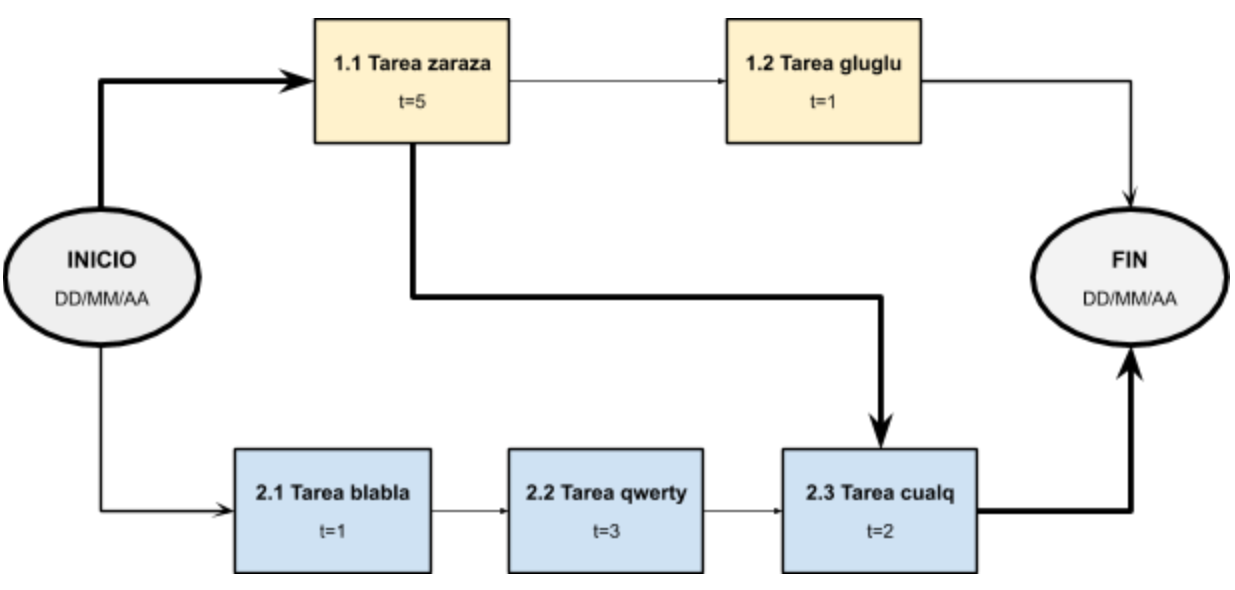
\includegraphics[width=.8\textwidth]{./Figuras/AoN.png}
            \caption{Diagrama de \textit{Activity on Node}.}
            \label{fig:AoN}
        \end{figure}

        Indicar claramente en qué unidades están expresados los tiempos.
        De ser necesario indicar los caminos semi críticos y analizar sus tiempos mediante un cuadro.
        Es recomendable usar colores y un cuadro indicativo describiendo qué representa cada color.

    \end{consigna}


    \section{11. Diagrama de Gantt}
    \label{sec:gantt}

    \begin{consigna}{red}
        Existen muchos programas y recursos \textit{online} para hacer diagramas de Gantt, entre los cuales destacamos:

        \begin{itemize}
            \item Planner
            \item GanttProject
            \item Trello + \textit{plugins}. En el siguiente link hay un tutorial oficial: \\ \url{https://blog.trello.com/es/diagrama-de-gantt-de-un-proyecto}
            \item Creately, herramienta online colaborativa. \\\url{https://creately.com/diagram/example/ieb3p3ml/LaTeX}
            \item Se puede hacer en latex con el paquete \textit{pgfgantt}\\ \url{http://ctan.dcc.uchile.cl/graphics/pgf/contrib/pgfgantt/pgfgantt.pdf}
        \end{itemize}

        Pegar acá una captura de pantalla del diagrama de Gantt, cuidando que la letra sea suficientemente grande como para ser legible.
        Si el diagrama queda demasiado ancho, se puede pegar primero la ``tabla'' del Gantt y luego pegar la parte del diagrama de barras del diagrama de Gantt.

        Configurar el software para que en la parte de la tabla muestre los códigos del EDT (WBS).\\
        Configurar el software para que al lado de cada barra muestre el nombre de cada tarea.\\
        Revisar que la fecha de finalización coincida con lo indicado en el Acta Constitutiva.

        En la figura \ref{fig:gantt}, se muestra un ejemplo de diagrama de gantt realizado con el paquete de \textit{pgfgantt}.
        En la plantilla pueden ver el código que lo genera y usarlo de base para construir el propio.

        Las fechas pueden ser calculadas utilizando alguna de las herramientas antes citadas. Sin embargo, el siguiente ejemplo
        fue elaborado utilizando
        \href{https://docs.google.com/spreadsheets/d/1fBz8NhSpc4tkkhz3KjJCbh1nR_ltDkfEcZi4tZXduqs}{esta hoja de cálculo}.

        Es importante destacar que el ancho del diagrama estará dado por la longitud del texto utilizado para las tareas
        (Ejemplo: tarea 1, tarea 2, etcétera) y el valor \textit{x unit}. Para mejorar la apariencia del diagrama, es necesario
        ajustar este valor y, quizás, acortar los nombres de las tareas.

        \begin{figure}[htpb]
            \begin{center}
                \begin{ganttchart}[
                    time slot unit=day,
                    time slot format=isodate,
                    x unit=0.038cm,
                    y unit title=0.7cm,
                    y unit chart=0.6cm,
                    milestone/.append style={xscale=4}
                ]{2021-03-05}{2021-12-16}
                    \gantttitlecalendar*{2021-03-05}{2021-12-16}{year} \\
                    \gantttitlecalendar*{2021-03-05}{2021-12-16}{month} \\
                    \ganttgroup{Duración Total}{2021-03-05}{2021-12-16} \\
                    %%%%%%%%%%%%%%%%%Organización
                    \ganttgroup{Organización}{2021-03-05}{2021-04-16} \\
                    \ganttbar{Planificación del proyecto}{2021-03-05}{2021-04-15} \\
                    %%%%%%%%%%%%%%%%%Ejecución
                    \ganttgroup{Ejecución}{2021-04-16}{2021-10-21} \\
                    \ganttbar{Tarea 1}{2021-04-16}{2021-04-29} \\
                    \ganttbar{Tarea 2}{2021-04-30}{2021-05-13} \\
                    \ganttbar{Tarea 3}{2021-05-14}{2021-05-27} \\
                    \ganttbar{Tarea 4}{2021-05-28}{2021-07-12} \\
                    \ganttbar{Tarea 5}{2021-07-13}{2021-08-09} \\
                    \ganttbar{Tarea 6}{2021-08-10}{2021-09-23} \\
                    \ganttbar{Tarea 7}{2021-09-24}{2021-09-30} \\
                    \ganttbar{Tarea 8}{2021-10-01}{2021-10-14} \\
                    \ganttbar{Tarea 9}{2021-10-15}{2021-10-21} \\
                    % %%%%%%%%%%%%%%%%%Finalización
                    \ganttgroup{Finalización}{2021-10-22}{2021-12-16} \\
                    \ganttbar{Memoria v1}{2021-10-22}{2021-11-04} \\
                    \ganttbar{Memoria v2}{2021-11-05}{2021-11-18} \\
                    \ganttbar{Memoria final}{2021-11-19}{2021-12-02} \\
                    % La fecha del siguiente milestone es la fecha en que terminamos la memoria
                    \ganttmilestone{Enviar memoria al director}{2021-12-02} \\
                    \ganttbar{Elaborar la presentación}{2021-12-03}{2021-12-16} \\
                    \ganttmilestone{Ensayo de la presentación}{2021-12-16} \\
                    %%%%%%%%%%%%%%%%%%%%%%%%%%%%%%%%%%%%%%%%%%%%%%%%%%%%%%%%%%%%%%%
                \end{ganttchart}
            \end{center}
            \caption{Diagrama de gantt de ejemplo}
            \label{fig:gantt}
        \end{figure}


        \begin{landscape}
            \begin{figure}[htpb]
                \centering
                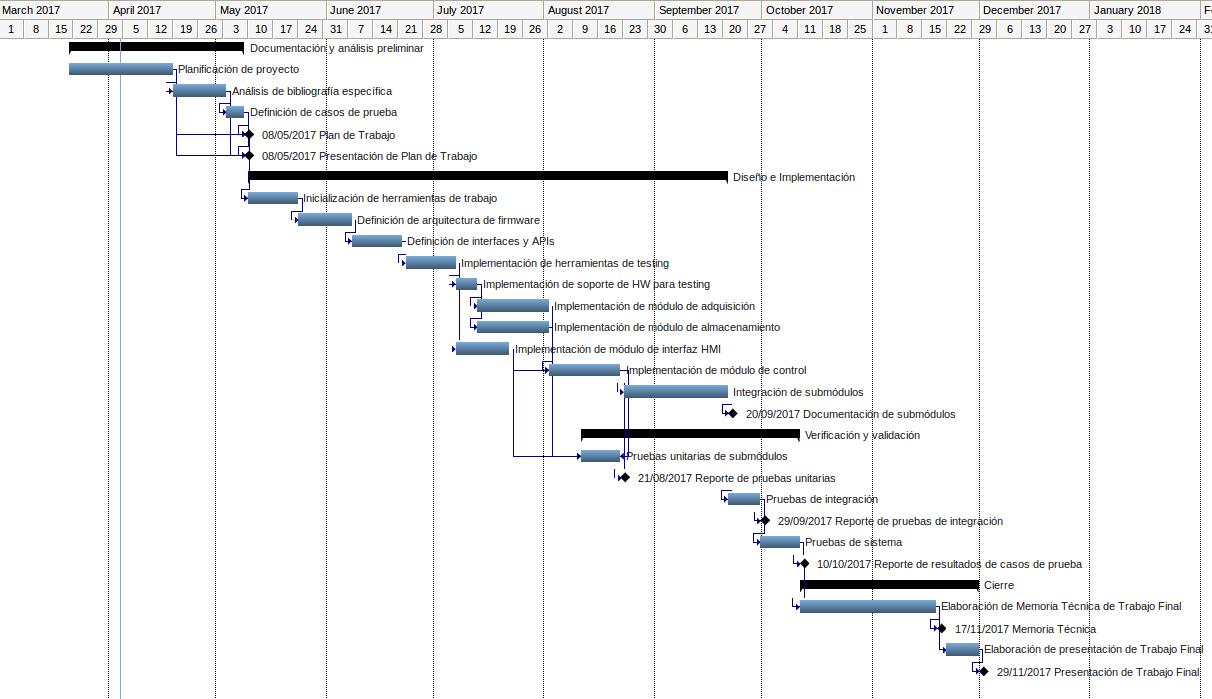
\includegraphics[height=.85\textheight]{./Figuras/Gantt-2.png}
                \caption{Ejemplo de diagrama de Gantt (apaisado).} %Modificar este título acorde.
                \label{fig:diagGantt}
            \end{figure}

        \end{landscape}

    \end{consigna}


    \section{12. Presupuesto detallado del proyecto}
    \label{sec:presupuesto}

    \begin{consigna}{red}
        Si el proyecto es complejo entonces separarlo en partes:
        \begin{itemize}
            \item Un total global, indicando el subtotal acumulado por cada una de las áreas.
            \item El desglose detallado del subtotal de cada una de las áreas.
        \end{itemize}

        IMPORTANTE: No olvidarse de considerar los COSTOS INDIRECTOS.

        Incluir la aclaración de si se emplea como moneda el peso argentino (ARS) o si se usa moneda extranjera (USD, EUR, etc). Si es en moneda extranjera se debe indicar la tasa de conversión respecto a la moneda local en una fecha dada.

    \end{consigna}

    \begin{table}[htpb]
        \centering
        \begin{tabularx}{\linewidth}{@{}|X|c|r|r|@{}}
            \hline
            \rowcolor[HTML]{C0C0C0}
            \multicolumn{4}{|c|}{\cellcolor[HTML]{C0C0C0}COSTOS DIRECTOS} \\ \hline
            \rowcolor[HTML]{C0C0C0}
            Descripción &
            \multicolumn{1}{c|}{\cellcolor[HTML]{C0C0C0}Cantidad} &
            \multicolumn{1}{c|}{\cellcolor[HTML]{C0C0C0}Valor unitario} &
            \multicolumn{1}{c|}{\cellcolor[HTML]{C0C0C0}Valor total} \\ \hline
            &
            \multicolumn{1}{c|}{} &
            \multicolumn{1}{c|}{} &
            \multicolumn{1}{c|}{} \\ \hline
            &
            \multicolumn{1}{c|}{} &
            \multicolumn{1}{c|}{} &
            \multicolumn{1}{c|}{} \\ \hline
            \multicolumn{1}{|l|}{} &
            &
            &
            \\ \hline
            \multicolumn{1}{|l|}{} &
            &
            &
            \\ \hline
            \multicolumn{3}{|c|}{SUBTOTAL} &
            \multicolumn{1}{c|}{} \\ \hline
            \rowcolor[HTML]{C0C0C0}
            \multicolumn{4}{|c|}{\cellcolor[HTML]{C0C0C0}COSTOS INDIRECTOS} \\ \hline
            \rowcolor[HTML]{C0C0C0}
            Descripción &
            \multicolumn{1}{c|}{\cellcolor[HTML]{C0C0C0}Cantidad} &
            \multicolumn{1}{c|}{\cellcolor[HTML]{C0C0C0}Valor unitario} &
            \multicolumn{1}{c|}{\cellcolor[HTML]{C0C0C0}Valor total} \\ \hline
            \multicolumn{1}{|l|}{} &
            &
            &
            \\ \hline
            \multicolumn{1}{|l|}{} &
            &
            &
            \\ \hline
            \multicolumn{1}{|l|}{} &
            &
            &
            \\ \hline
            \multicolumn{3}{|c|}{SUBTOTAL} &
            \multicolumn{1}{c|}{} \\ \hline
            \rowcolor[HTML]{C0C0C0}
            \multicolumn{3}{|c|}{TOTAL} &
            \\ \hline
        \end{tabularx}%
    \end{table}


    \section{13. Gestión de riesgos}
    \label{sec:riesgos}

    \begin{consigna}{red}
        a) Identificación de los riesgos (al menos cinco) y estimación de sus consecuencias:

        Riesgo 1: detallar el riesgo (riesgo es algo que si ocurre altera los planes previstos de forma negativa)
        \begin{itemize}
            \item Severidad (S): mientras más severo, más alto es el número (usar números del 1 al 10).\\
            Justificar el motivo por el cual se asigna determinado número de severidad (S).
            \item Probabilidad de ocurrencia (O): mientras más probable, más alto es el número (usar del 1 al 10).\\
            Justificar el motivo por el cual se asigna determinado número de (O).
        \end{itemize}

        Riesgo 2:
        \begin{itemize}
            \item Severidad (S): X.\\
            Justificación...
            \item Ocurrencia (O): Y.\\
            Justificación...
        \end{itemize}

        Riesgo 3:
        \begin{itemize}
            \item Severidad (S): X.\\
            Justificación...
            \item Ocurrencia (O): Y.\\
            Justificación...
        \end{itemize}


        b) Tabla de gestión de riesgos:      (El RPN se calcula como RPN=SxO)

        \begin{table}[htpb]
            \centering
            \begin{tabularx}{\linewidth}{@{}|X|c|c|c|c|c|c|@{}}
                \hline
                \rowcolor[HTML]{C0C0C0}
                Riesgo & S & O & RPN & S* & O* & RPN* \\ \hline
                &   &   &     &    &    &      \\ \hline
                &   &   &     &    &    &      \\ \hline
                &   &   &     &    &    &      \\ \hline
                &   &   &     &    &    &      \\ \hline
                &   &   &     &    &    &      \\ \hline
            \end{tabularx}%
        \end{table}

        Criterio adoptado:

        Se tomarán medidas de mitigación en los riesgos cuyos números de RPN sean mayores a...

        Nota: los valores marcados con (*) en la tabla corresponden luego de haber aplicado la mitigación.

        c) Plan de mitigación de los riesgos que originalmente excedían el RPN máximo establecido:

        Riesgo 1: plan de mitigación (si por el RPN fuera necesario elaborar un plan de mitigación).
        Nueva asignación de S y O, con su respectiva justificación:
        \begin{itemize}
            \item Severidad (S*): mientras más severo, más alto es el número (usar números del 1 al 10).
            Justificar el motivo por el cual se asigna determinado número de severidad (S).
            \item Probabilidad de ocurrencia (O*): mientras más probable, más alto es el número (usar del 1 al 10).
            Justificar el motivo por el cual se asigna determinado número de (O).
        \end{itemize}

        Riesgo 2: plan de mitigación (si por el RPN fuera necesario elaborar un plan de mitigación).

        Riesgo 3: plan de mitigación (si por el RPN fuera necesario elaborar un plan de mitigación).

    \end{consigna}


    \section{14. Gestión de la calidad}
    \label{sec:calidad}

    \begin{consigna}{red}
        Elija al menos diez requerimientos que a su criterio sean los más importantes/críticos/que aportan más valor y para cada uno de ellos indique las acciones de verificación y validación que permitan asegurar su cumplimiento.

        \begin{itemize}
            \item Req \#1: copiar acá el requerimiento con su correspondiente número.

            \begin{itemize}
                \item Verificación para confirmar si se cumplió con lo requerido antes de mostrar el sistema al cliente. Detallar.
                \item Validación con el cliente para confirmar que está de acuerdo en que se cumplió con lo requerido. Detallar.
            \end{itemize}

        \end{itemize}

        Tener en cuenta que en este contexto se pueden mencionar simulaciones, cálculos, revisión de hojas de datos, consulta con expertos, mediciones, etc.

        Las acciones de verificación suelen considerar al entregable como ``caja blanca'', es decir se conoce en profundidad su funcionamiento interno.

        En cambio, las acciones de validación suelen considerar al entregable como ``caja negra'', es decir, que no se conocen los detalles de su funcionamiento interno.

    \end{consigna}


    \section{15. Procesos de cierre}
    \label{sec:cierre}

    \begin{consigna}{red}
        Establecer las pautas de trabajo para realizar una reunión final de evaluación del proyecto, tal que contemple las siguientes actividades:

        \begin{itemize}
            \item Pautas de trabajo que se seguirán para analizar si se respetó el Plan de Proyecto original:\\
            - Indicar quién se ocupará de hacer esto y cuál será el procedimiento a aplicar.
            \item Identificación de las técnicas y procedimientos útiles e inútiles que se emplearon, los problemas que surgieron y cómo se solucionaron:\\
            - Indicar quién se ocupará de hacer esto y cuál será el procedimiento para dejar registro.
            \item Indicar quién organizará el acto de agradecimiento a todos los interesados, y en especial al equipo de trabajo y colaboradores:\\
            - Indicar esto y quién financiará los gastos correspondientes.
        \end{itemize}

    \end{consigna}

\end{document}
